%
% $File: report.tex
% $Date: Sun Dec 01 21:22:10 2013 +0800
%

\documentclass{article}
\usepackage{fontspec}
\usepackage{zhspacing,url,amsmath,amssymb,verbatim}
\usepackage{pdfpages}
\zhspacing
\usepackage{listings}
\usepackage[hyperfootnotes=false,colorlinks,linkcolor=blue,anchorcolor=blue,citecolor=blue]{hyperref}
\usepackage[backend=biber]{biblatex}
\usepackage{graphicx}
\usepackage{minted}
\usepackage{subfigure}
\usepackage{indentfirst}
\usepackage{cases}
\usepackage{environ}
\usepackage{array}
\usepackage[top=1in, bottom=1in, left=1.25in, right=1.25in]{geometry}
\usepackage{caption}
%\usepackage{tikz}
%\usepackage{dot2texi}

% $File: mint-defs.tex
% $Date: Sun Nov 17 23:37:24 2013 +0800
% $Author: Xinyu Zhou <zxytim@gmail.com>

\newcommand{\inputmintedConfigured}[3][]{\inputminted[fontsize=\footnotesize,
	label=#3,linenos,frame=lines,framesep=0.8em,tabsize=4,#1]{#2}{#3}}

\newcommand{\txtsrc}[2][]{\inputmintedConfigured[#1]{text}{#2}}
\newcommand{\txtsrcpart}[4][]{\txtsrc[firstline=#3,firstnumber=#3,lastline=#4,#1]{#2}}

\newcommand{\cppsrc}[2][]{\inputmintedConfigured[#1]{cpp}{#2}}
\newcommand{\cppsrcpart}[4][]{\cppsrc[firstline=#3,firstnumber=#3,lastline=#4,#1]{#2}}

\newcommand{\javasrc}[2][]{\inputmintedConfigured[#1]{java}{#2}}
\newcommand{\javasrcpart}[4][]{\javasrc[firstline=#3,firstnumber=#3,lastline=#4,#1]{#2}}

\newcommand{\matlabsrc}[2][]{\inputmintedConfigured[#1]{matlab}{#2}}
\newcommand{\matlabsrcpart}[4][]{\matlabsrc[firstline=#3,firstnumber=#3,lastline=#4,#1]{#2}}

\newcommand{\pysrc}[2][]{\inputmintedConfigured[#1]{matlab}{#2}}
\newcommand{\pysrcpart}[4][]{\matlabsrc[firstline=#3,firstnumber=#3,lastline=#4,#1]{#2}}

%\usepackage[T1]{fontenc}
\usepackage{lmodern}
\usepackage{amssymb,amsmath}
\usepackage{ifxetex,ifluatex}
\usepackage{fixltx2e} % provides \textsubscript
% use upquote if available, for straight quotes in verbatim environments
\IfFileExists{upquote.sty}{\usepackage{upquote}}{}
\ifnum 0\ifxetex 1\fi\ifluatex 1\fi=0 % if pdftex
  \usepackage[utf8]{inputenc}
\else % if luatex or xelatex
  \usepackage{fontspec}
  % commented by Xinyu Zhou
  \ifxetex
    \usepackage{xltxtra,xunicode}
  \fi
  \defaultfontfeatures{Mapping=tex-text,Scale=MatchLowercase}
  \newcommand{\euro}{€}
\fi
% use microtype if available
\IfFileExists{microtype.sty}{\usepackage{microtype}}{}
\usepackage{color}
\usepackage{fancyvrb}
\newcommand{\VerbBar}{|}
\DefineShortVerb[commandchars=\\\{\}]{\|}
\DefineVerbatimEnvironment{Highlighting}{Verbatim}{commandchars=\\\{\}}
% Add ',fontsize=\small' for more characters per line
\newenvironment{Shaded}{}{}
\newcommand{\KeywordTok}[1]{\textcolor[rgb]{0.00,0.44,0.13}{\textbf{{#1}}}}
\newcommand{\DataTypeTok}[1]{\textcolor[rgb]{0.56,0.13,0.00}{{#1}}}
\newcommand{\DecValTok}[1]{\textcolor[rgb]{0.25,0.63,0.44}{{#1}}}
\newcommand{\BaseNTok}[1]{\textcolor[rgb]{0.25,0.63,0.44}{{#1}}}
\newcommand{\FloatTok}[1]{\textcolor[rgb]{0.25,0.63,0.44}{{#1}}}
\newcommand{\CharTok}[1]{\textcolor[rgb]{0.25,0.44,0.63}{{#1}}}
\newcommand{\StringTok}[1]{\textcolor[rgb]{0.25,0.44,0.63}{{#1}}}
\newcommand{\CommentTok}[1]{\textcolor[rgb]{0.38,0.63,0.69}{\textit{{#1}}}}
\newcommand{\OtherTok}[1]{\textcolor[rgb]{0.00,0.44,0.13}{{#1}}}
\newcommand{\AlertTok}[1]{\textcolor[rgb]{1.00,0.00,0.00}{\textbf{{#1}}}}
\newcommand{\FunctionTok}[1]{\textcolor[rgb]{0.02,0.16,0.49}{{#1}}}
\newcommand{\RegionMarkerTok}[1]{{#1}}
\newcommand{\ErrorTok}[1]{\textcolor[rgb]{1.00,0.00,0.00}{\textbf{{#1}}}}
\newcommand{\NormalTok}[1]{{#1}}
% \ifxetex
%   \usepackage[setpagesize=false, % page size defined by xetex
%               unicode=false, % unicode breaks when used with xetex
%               xetex]{hyperref}
% \else
%   \usepackage[unicode=true]{hyperref}
% \fi
\hypersetup{breaklinks=true,
            bookmarks=true,
            pdfauthor={},
            pdftitle={},
            colorlinks=true,
            urlcolor=blue,
            %linkcolor=magenta,
            pdfborder={0 0 0}}
%\urlstyle{same}  % don't use monospace font for urls
\setlength{\parindent}{0pt}
\setlength{\parskip}{6pt plus 2pt minus 1pt}
\setlength{\emergencystretch}{3em}  % prevent overfull lines
%\setcounter{secnumdepth}{0}



\newcommand{\figref}[1]{\hyperref[fig:#1]{Figure\ref*{fig:#1}}}
\newcommand{\tableref}[1]{\hyperref[table:#1]{Table\ref*{table:#1}}}
\newcommand{\centerize}[1]{\begin{center} #1 \end{center}}

\newcommand{\cmd}[1]{{\it #1}}
\newcommand{\ccmd}[1]{\centerize{\cmd{#1}}}

\title{Digital Signal Processing: Speaker Recognition \\ Midterm Report}
\author{Xinyu Zhou, Yuxin Wu, and Tiezheng Li\\ Tsinghua University}
\date{}

\bibliography{refs.bib}
\begin{document}

\fontsize{11pt}{1.4em}
\setlength{\baselineskip}{1.6em}
\maketitle

\section{Task}
	Build a speaker recognition system

\section{Dataset}
	The dataset provided by teacher comprised of 102 speaker, in which 60 are
	females and the rest are males, with three different speaking style: Spontaneous,
	Reading and Whisper. A statistic is as follows:
	\begin{table}[!ht]
		\centering
		\begin{tabular}{|c|c|c|c|}
			\hline
			& Spontaneous & Reading & Whisper \\\hline
			Average Duration & 202s & 205s & 221s \\\hline
			Female Average Duration & 205s & 202s & 217s \\\hline
			Male Average Duration & 200s & 203s & 223s \\\hline
		\end{tabular}
	\end{table}

\section{Approach}

Based on weeks of literature reviewing and testing,
we have designed our overall approach to this task as followed:

\begin{enumerate}
    \item Energy-Based VAD

      Input audio signals are very likely to contain significantly large ratio of blank signals.
      VAD (Voice Activity Detector)
      is a preprocessing technique to filter out the blank period.
      The most common approach toward this goal is to use energy-based feature of signals.

      \item Cepstrum-Based Features

        Research showed that cepstrum-based features are more discrimitive in the task of speech and speaker recognition/verification.
        We decide to apply common cepstrum features extraction routine, such as MFCC (Mel-frequency Cepstrum Coefficients), LFCC,
        after the original signals are preprocessed by VAD.

       The basic procedure of MFCC is shown below, and the details about
       extracting MFCC is already been explained in the previous reports.
       The output of this step, is a sequence of fixed-dimension vectors, which will be used later in model training.

      \begin{figure}[H]
        \centering
        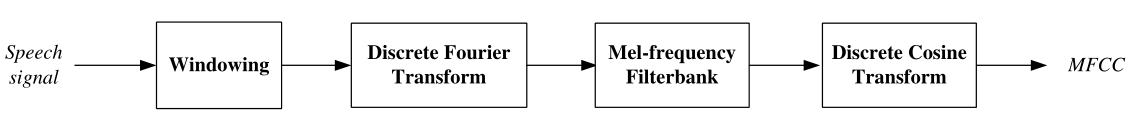
\includegraphics[width=\textwidth]{res/MFCC.png}
      \end{figure}

    \item GMM and UBM Model

      Since the feature vectors of a speaker tend to cluster into \textbf{several} groups
      in the feature space,
      the model of a specific speaker can be well described by using GMM (Gaussian Mixture Model).
      Moreover, for different speakers, the components of their individual GMMs
      will also have similar distributions, which discriminate different syllables.
      Therefore, an UBM (Universal Background Model) can be first trained for all speakers,
      and then we can get adapted GMMs which fit this task better.

      \begin{figure}[H]
        \centering
        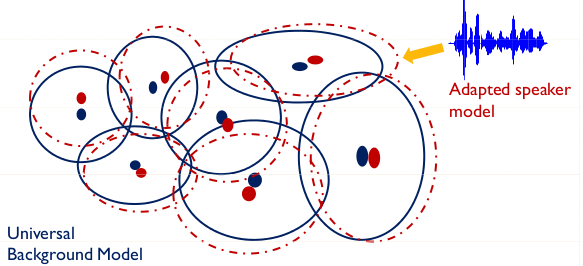
\includegraphics[width=0.7\textwidth]{res/ubm.png}
      \end{figure}

      \item JFA
        GMM-based model can describe the clusterred distribution, but it fails to account for
        different types of variability in each clusterred group.
        However, we only need inter-speaker variability to be modeled,
		but not channel or noise variability. Join Factor Analysis can convey
		such information.

  \end{enumerate}



\section{Progress}
	Till now, we have implemented MFCC feature extractor and GMM model for
	acoustic modeling. For GMM we employ scikit-learn\cite{scikit-learn}.

	We've tested on 20 speakers for a closed set recognition task and calculate
	accuracy of recognition. 30 seconds utterance is used for training, and 5
	seconds utterance is used for test. We randomly extract 100 continuous 5-second
	test utterance from utterance of a speaker as test set.
	There's no overlap between training and test utterance.

	For the last week, we fine-tuned parameters of our model and scrutinizing more
	paper preceding to our work.

	The test is repeated 20 times to obtain an accurate estimate of accuracy.
	The test result is as follows:

	\begin{itemize}
		\item \textbf{Spontaneous} 0.940
		\item \textbf{Reading} 0.926
		\item \textbf{Whisper} 0.931
	\end{itemize}

\section{Analysis}
	The result indicates the effectiveness of our method, but also shows the limitation.
	\begin{enumerate}
		\item The performance is not satisfying. \\
			Compare to the performance given in serval sources (books and papers),
			ours are not the best.  This may due to the corpus difference between
			test, and the result may not be comparable.
			But comparing to MFCC extractor provided by
			bob\cite{bob2012}, we get $5\%$ higher accuracy, which proved the
			effectiveness of our model.
		\item Long training utterance. \\
			30s utterance training data may not feasible in practical application.
		\item GMM is of low efficiency when classifying. \\
			Due to the modeling of each spkeaker using GMM with 32 mixtures,
			classification of a single speaker involves scoring over all
			enrolled speakers. The more speaker, the less efficiency.
	\end{enumerate}


\section{Future Work}
In the following two weeks, we plan to:

\begin{enumerate}
	\item Compare performance with other algorithms on the same corpus.\\
		Comparison is of importance since it gives us vital feedback on our approach.
	\item Reduce test utterance length. \\
		5s utterance after VAD can be reduced to make our approach more applicable.
	\item Employ GMM-UBM to get more accurate GMM model.
	\item understanding JFA.
	\item Extend our method to open set recognition.
	\item GUI functional design.
\end{enumerate}

Moreover, we've proposed some other methods which need futher investigation:
\begin{enumerate}
	\item using Bootstraped-Multi-GMM to convey more information.
\end{enumerate}


\printbibliography

\end{document}

